\section{Transfer Learning}
In this section, we first describe the intuition behind transfer learning.
Then, we elaborate the details of our transfer learning based approach with running examples.

\subsection{Knowledge Transfer}
In our case, the use of transfer learning is motivated by the fact that people often have one or only a few buildings labeled which they want to take advantage of to aid the labeling of a new buidlings.
Transfer learning fits such a scenario well in that it exploits knowledge gained from one domain\footnote{A ``domain'' particularly refers to a data set  in this paper.} where labeled data is abundant to help classify examples in a new related domain. 
Such knowledge transfer is possible when the training domain and the test domain have the same set of class labels. 
In our sensor type classfication setting, we assume that we are provided with some labeled examples only from the training domain but do not have any labeled ones from the testing domain. 
The reason that traditional supervised learning techniques is not successful in transferring knowledge across domains in our case is because it usually requires the training and the testing examples sampled i.i.d. from the same distribution, which is not the case for our problem.

%For example, the classiers can be trained from several relevant domains or built using different learning algorithms on the same domain.
Based on the observation in Section x.x that classifers constructed with data features perform better than name features, we construct a few classifiers with different learning algorithms on the same set of data features from an existing building. 
Each different classifier usually contains a different perspective of the knowledge on the building, due to the inductive bias of the specific learning model. 
We refer to these different classifiers as {\it base} models and will combine them for classification on the new building.

\subsection{Locally Weighted Ensemble}
Different models can be effective at diffrent regions or structures in the new testing building, and no single model can perform well on all examples. 
Ideally, we want to combine the knowledge in the base models, rather than only using any particular model, to more effectively transfer the knowledge to the new building. A natural choice is model averaging that additively combines the predictions of multiple base learners. 
However, the existing model averaging methods for traditional supervised learning usually assign global weights to models, which are either uniform (e.g., in Bagging~\cite{bagging}) or proportional to the training accuracy (e.g., in Boosting~\cite{boosting}), or simply relying on a specific model (e.g., single model classification).
Such global weighting schemes may not perform well in transfer learning because different testing examples may favor predictions from different base models. 
For example, when the base models carry conflicting concepts at a testing example, it is essential to select the model that better represents the distribution underlying the example.

We employ a locally weighted ensemble~\cite{lwe} to weight the predictions from each base classifier. The weight is computed per model per example based on the similarity between the model and the local structure of the target example. The similarity is measured by comparing neighborhood graphs which we will explain in the next section. Such local weighting will prefer models whose predicted local structure is close to the true local structure of the target example in the new testing domain. Let $x$ be the data feature vector of an example in the new building and $y$ be its predicted class label. Given a set of k base models $M_1$,..., $M_k$ and the new testing set $D_T$ represented with the data feature view, the general Bayesian model averaging rule to estimate the posterior distribution of y is,
\begin{equation}\label{lwe}
p(y|x)=\sum_{i=1}^k p(y|x,D_T,M_i) p(M_i|D_T)
\end{equation}
where $p(y|x,D_T,M_i) = p(y|x,M_i)$ because $x \in D_T$ and $p(y|x,M_i)$ is actually the prediction on $x$ by $M_i$. And $p(M_i|D_T)$ is the probability to choose $M_i$ given the testing set $D_T$. As $x \in D_T$, $p(M_i|D_T)$ equals to $p(M_i|x)$ which is the locally adjusted weight for $M_i$ and Eq.~\ref{lwe} becomes,
\begin{equation}\label{sum}
p(y|x)=\sum_{i=1}^k w_{x}^{M_i} p(y|x, M_i)
\end{equation}
where $w_{x}^{M_i} = p(M_i|x)$ and intuitively, a model $M_i$ should have higher weights for $x$ if $M_i$ predicts a similar local structure of $x$ to the true one.
We will next explain how the weight is calculated per example.

\subsection{Graph-based Weight Estimation}
If $p(y|x)$ is known, we can estimate the weights $w_{x}^{M_i}$ for each model by minimizing the square error between its prediction and the ground truth. 
However, in practice the truth value of $p(y|x)$ for a new building is not available a priori . 
The main task becomes to properly define the similarity between classifier's predicted structure and the true structure. 
Based on the clustering assumption~\cite{cluster} that $p(y|x)$ is not expected
to change much in a dense area where $p(x)$ is high, which means the decision boundary probably exists in areas with smaller $p(x)$.
Therefore, we perform clustering on the new testing set and assume the boundries between clusters represent areas where $p(x)$ is small.
If the clustering boundary for the region where $x$ locates agrees with the decision boundary of $M_i$, we assume that $p(y|x,M_i)$ is similar to the true $p(y|x)$ around $x$, which means we can assign a larger weight to $Mi$ at $x$. 
In other words, if the predicitons of $M_i$ on the area surrounding $x$ have higher consistency with the clustering results, $M_i$ would have a larger weight at $x$. 

Following these observations, we employ a graph-based algorithm to compute the weight.
To compute the $w_{x}^{M_i}$ for $M_i$ at example $x$, we construct two neighorhood graphs: 
$G_M = (V, E_M)$ and $G_C = (V, E_C)$, for classification and clustering respectively, 
where each vertex is an example and $V = D_T$. In $G_M$, an edge exists between two vertices (denoting the two examples are ``neighbors'') if and only if an $M_i$ predicts the same label for these two examples. Likewise, in $G_C$, an edge exists between two vertices if and only if these two examples reside in the same cluster.
If $x$ neighborhs on both graphs have significant overlap, then $M_i$ will be assigned a larger weight.
So the weight $w_{x}^{M_i}$ for $M_i$ at $x$ is proportional to the similarity of the two graphs:
\begin{equation}\label{sim}
w_{x}^{M_i} \propto s(G_M, G_C|x) = \frac {|V_M \cap V_C|} {|V_M \cup V_C|}
\end{equation}
where $V_M$ ($V_C$) is the set of neighbors of $x$ on graph $G_M$ ($G_C$), |$\cdot$| is the cardinality of a set, and $s(G_M, G_C|x)$ is the similarity of between two graphs. 
Figure~\ref{fig:graph} illustrates an example of neighborhood graphs for an example $x$ (in grey circle): model 1 has a similarity of 0.75 while model 2 has 0.4.

\begin{figure}[h]
\centering
    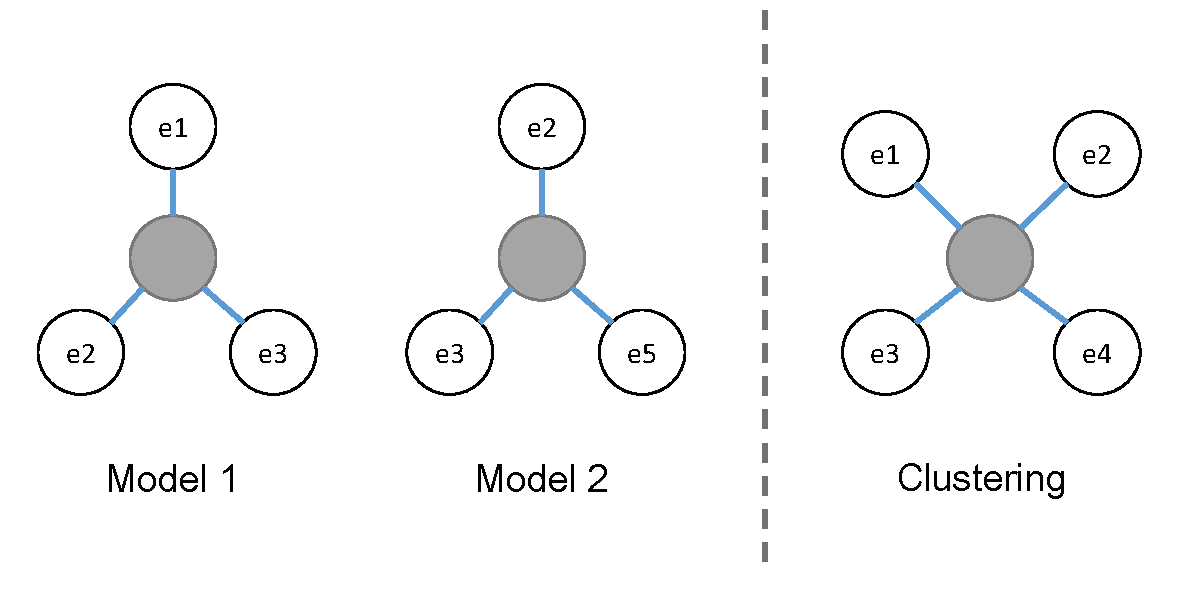
\includegraphics[width=0.45\textwidth]{./fig/lwe_graph}
\caption{An example of local neighborhood graphs of $x$ (in grey circle).}
\label{fig:graph}
\end{figure}

With the eq.~\ref{sim} defined, we can compute the weight for each $M_i$ by normalizing among all similarity scores:
\begin{equation}\label{sim}
w_{x}^{M_i} = \frac {s(G_{M_i}, G_C|x)} {\sum_{i=1}^k s(G_{M_i}, G_C|x)}
\end{equation}
And the final prediction for $x$ is simply $\hat y = argmax_y \enspace p(y|x)$ as $p(y|x)$ is defined in Eq.\label{lwe}.

\subsubsection{Distance-based correction}
We notice if considering the distance between examples as shown in Figure~\ref{graph_dist}, the original similarity definition is problematic in that both models will be assigned the same weight while obviously model 2 ought to have a higher weight because the neighbors are closer to the target example.
As a correction to include the distance between examples into consideration, the adjusted similarity is:
\begin{equation}\label{sim}
s\ast(G_M, G_C|x) = 1 - \frac {\sum d_{V_I}/|V_I|} {\sum d_{V_U}/|V_U|}
\end{equation}
where $V_I = V_M \cap V_C$, $V_U = V_M \cup V_C$, and $\sum d_{V_I}$ is the sum of distance between $x$ to its neighbors in $V_I$ (likewise for $\sum d_{V_U}$).

\begin{figure}[h]
\centering
    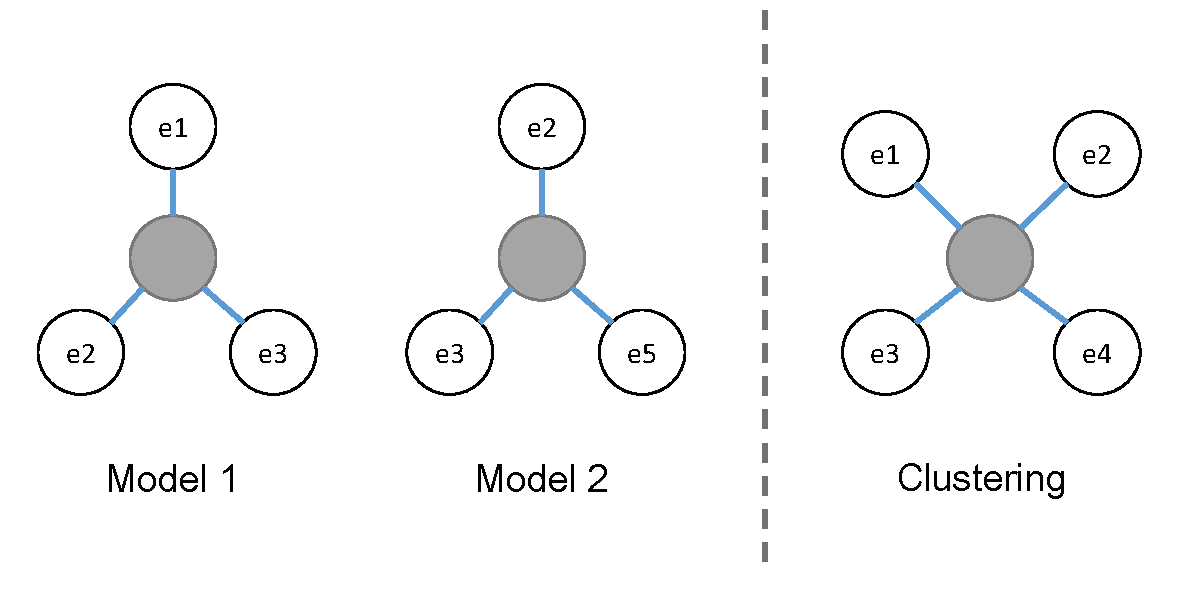
\includegraphics[width=0.45\textwidth]{./fig/lwe_graph}
\caption{An example of local neighborhood graphs of $x$ with distance into consideration.}
\label{graph_dist}
\end{figure}

\subsection{Clustering with Non-parametric Bayesian}
\label{sec_clustering}
In our transfer learning based approach, data density $p(x)$ is exploited via its latent clustering structure. We choose Gaussian Mixture Model (GMM) \cite{zivkovic2004improved}, a partitional clustering algorithm, to perform the clustering.

In GMM, the cluster label for every instance is treated as a latent variable, which is drawn from a multinomial distribution $p(c)$, i.e., $p(c)\propto\alpha_c$, where $\forall c, \alpha_c\ge0$ and $\sum_c\alpha_c=1$. In any given cluster $c$, the conditional data likelihood of an instance $x$ is specified by a multivariate Gaussian distribution. To reduce the number of parameters to estimate, we choose the isotropic Gaussian in our solution,
\begin{equation}
p(x|c)=(2\pi\sigma^2)^{-d/2}\exp{-\frac{(x-\mu_c)^\mt(x-\mu_c)}{2\sigma^2}}
\end{equation}
where the variance $\sigma^2$ is shared by all the clusters. $\{\alpha_c, \mu_c\}^k_{c=1}$ and $\sigma$ are considered as model parameters in GMM.

However, in GMM, we need to manually specify the number of clusters for a given input data set; and the clustering result of GMM is very sensitive to such setting. More importantly, in our study, usually there is more than one pattern in the point names even for the same type of sensors; therefore we cannot assume one class has only one cluster. It is impossible for us to predefine those optimal cluster sizes. To make clustering feasible on the new building, we appeal to a non-parameter Bayesian solution: we assume the model parameters $(\alpha, \mu)$ in each cluster are also random variables, which are drawn from a Dirichlet Process prior \cite{dp}.

A Dirichlet Process $DP(G_0, \eta)$ with a base distribution $G_0$ and a scaling parameter $\eta$ is a distribution over distributions~\cite{dp}. The base distribution $G_0$ specifies the prior distribution of model parameters, e.g., mean parameter $\mu$ in each cluster, and the scaling parameter $\eta$ specifies the concentration of samples drawn from the DP, e.g., cluster proportion $p(c)$. An important property of the DP is that though the draws from a DP have countably infinite size, they are discrete with probability one, which leads to a probability distribution on partitions of the data. The number of unique draws, i.e., the number of clusters, varies with respect to the data and therefore is random, instead of being pre-specified.

As a result, with the introduced $DP(G_{0}, \eta)$ prior, data density in a given collection of instances can be expressed using a stick-breaking representation
\cite{sethuraman1994constructive}:
\begin{equation}\label{eq_dp_density}
p(x)=\sum_{c=1}^\infty \alpha_c \mathcal{N}(x|\mu_c,\sigma)p(\mu_c|G_0)
\end{equation}
where $\alpha={\alpha}_{c=1}^\infty\sim Stick(\eta)$ represents the proportion of clusters in the whole collection. The stick-breaking process $Stick(\eta)$ for the cluster proportion parameter $\alpha$ is defined as: $\alpha'_c\sim Beta(1, \eta), \alpha_c=\alpha'_c\prod_{i=1}^{c-1}(1-\alpha'_i)$. Since the variance $\sigma^2$ is fixed in all clusters, we use a conjugate prior for $\mu$ in $G_0$, i.e., for $\forall c, \mu_{ci}\sim \mathcal{N}(a,b)$, with the assumption that each dimension in $\mu_c$ is independently drawn from a univariate Gaussian. This will greatly simplify the later on inference procedure.

Because the data density distribution defined in Eq~\eqref{eq_dp_density} only has finite support at the points of $\{\alpha_c, \mu_c\}^k_{c=1}$, we can calculate the posterior distribution of latent cluster labels in each unlabeled instance to discover the clustering structure. Following the sampling scheme proposed in \cite{neal2000markov}, we appeal to a Gibbs sampling method to infer the posterior of cluster membership. Detailed specifications of this sampling algorithm can be found in \cite{neal2000markov}.

\subsubsection{Features for Clustering}
We use point name features to generate clusters for the new building. In general, point names following the same pattern would not vary too much, which will yield clusters of higher quality than data features.
Table~\ref{quality} shows the quality of clusters generated by DP with data features and name features measured by rand index~\cite{rand}. Rand index is a standard measure of the similarity between the grouping in clusters and the true labels.

\begin{table}[h]
\centering
\begin{tabular}{l|c|c}
\hline
                & Data Feature & Name Feature \\ \hline
Rand Index & 0.34       & 0.75       \\ \hline
\end{tabular}
\caption{Quality of clusters generated with different features measure by rand index (in the range [0,1], higher is better).}
\label{table:clf}
\end{table}

{\bf Putting it all together:} Algorithm~\ref{algo} summarizes our  tranfer learning based solution for the sensor type classification. FIX: algorithm and a quick sum here.

\begin{algorithm}[ht]
 \caption{Clustering-based Active Learning}
 \label{algo}
 %\SetAlgoLined
 {\bf Input}: point names $\mathcal{D}=\{x_1,x_2,\dots,x_n\}$, and label budget $B$\\
 {\bf Output}: predicted labels of the point names $Y$\\
 Initialize: Generate clusters with $DP(G_{0}, \eta)$ on $\mathcal{D}$, reset the labeled instance set $\mathcal{D}_l$ and propagated label set $\mathcal{D}_p$ to empty\\
\While{$B>0$}{
Train classifier $f(x)\to y$ based on $\mathcal{D}_l$ and $\mathcal{D}_p$\;
Apply $f(x)$ to all instances in $\mathcal{D}$\;
Compute class entropy $H(c)$ defined in Eq~\eqref{eq_entropy} for each cluster $c$\;
Retrieve a cluster by $\hat c=\argmax_c p(c)H(c)$\;
Acquire label $\hat y$ for example $\hat x$ given by $\argmax_{x\in\mathcal{D}} Pr(x|\hat c)$, and move $(\hat x, \hat y)$ from $\mathcal{D}$ to $\mathcal{D}_l$\;
Update the distance threshold $r$ by Eq~\eqref{eq_threshold}\;
Update all previous propagated label in $\mathcal{D}_p$ with new threshold $r$\;
Assign $\hat y$ to all unlabeled examples $x_{u}$, where $x_{u} \in \hat c$ and $d(x_u,\hat x)<r$\;
Move $(x_u, y)$ from $\mathcal{D}$ to $\mathcal{D}_p$\;
Perform sub-clustering with $DP(G_0, \eta)$ in $\hat c$\;
}
\end{algorithm}
